%!TEX TS-program = xelatex
\documentclass[]{friggeri-cv}
\usepackage{afterpage}
\usepackage{color}
\usepackage{xcolor}
\usepackage{hyperref}
\hypersetup{
    pdftitle={},
    pdfauthor={},
    pdfsubject={},
    pdfkeywords={},
    colorlinks=false,       % no lik border color
   allbordercolors=white    % white border color for all
}
\addbibresource{bibliography.bib}
\RequirePackage{xcolor}
\definecolor{pblue}{HTML}{0395DE}

\begin{document}
\header{\hspace{3.0cm} Rogério }{Jorge 12/04/1992}
      %{\hspace{3.0cm}Rogério Manuel Cabete de Jesus Jorge, April 12, 1992}
      
% Fake text to add separator      
\fcolorbox{white}{gray}{\parbox{\dimexpr\textwidth-2\fboxsep-2\fboxrule}{%
.....
}}

% In the aside, each new line forces a line break
\begin{aside}
  \section{Address}
    \textbf{Switzerland}
    Chemin des Uttins, 19 1028, Préverenges, Lausanne, Switzerland
    ~
    \textbf{Portugal}
    Avenida Almirante Reis, 56 1170, Lisboa, Portugal
    ~
    Rua da Escola, nº23 2º direito, Chã-Tavarede, Figueira da Foz, Portugal
    ~
  \section{Tel}
    +351 920520221 (PT)
    +41 0765074111 (CH)
    ~
  \section{Mail}
    \href{mailto:rogeriodejesusjorge@gmail.com}{\textbf{rogeriodejesusjorge@}\\gmail.com}
    \href{mailto:rogerio.jorge@epfl.ch}{\textbf{rogerio.jorge@}\\epfl.ch}
    \href{mailto:rogerio.jorge@ist.pt}{\textbf{rogerio.jorge@}\\ist.pt}
    ~
  \section{Web \& Git}
    \href{http://web.ist.utl.pt/~rogerio.jorge}{web.ist.utl.pt\\/\char`\~rogerio.jorge}
    \href{https://github.com/rogeriodejesusjorge}{github.com\\/rogeriodejesusjorge}
    %~
  %\section{Programming}
    %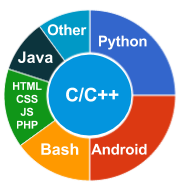
\includegraphics[scale=0.62]{img/programming.png}
    %~
  %\section{OS Preference}
    %\textbf{GNU/Linux}
\includegraphics[scale=0.40]{img/5stars.png}
    %\textbf{Unix}
\includegraphics[scale=0.40]{img/4stars.png}
    %\textbf{MacOS}
\includegraphics[scale=0.40]{img/2stars.png}
    %\textbf{Windows}
\includegraphics[scale=0.40]{img/1stars.png}
    %~
  %\section{Personal Skills}
    %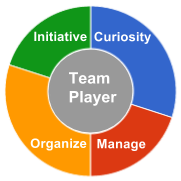
\includegraphics[scale=0.62]{img/personal.png}
    ~
  \section{Research Topics}
    %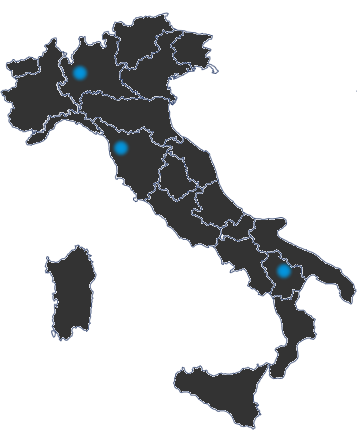
\includegraphics[scale=0.25]{img/italia.png}
    \textbf{Plasma Physics}
    Magnetic Confinement
    Tokamak Edge (SOL)
    \textbf{General Relativity}
    Black Holes
    General Relativistic MHD
    ~
  \section{Languages}
    \textbf{Portuguese}
\includegraphics[scale=0.40]{img/5stars.png}
    \textbf{English}
\includegraphics[scale=0.40]{img/4stars.png}
    \textbf{French}
\includegraphics[scale=0.40]{img/2stars.png}
    Matlab/Mathematica
    Latex/Fortran
    HTML/CSS/PHP/MySQL
\end{aside}

\section{Experience}
\begin{entrylist}
  \entry
    {01/15 - Now}
    {PhD Student}
    {\\
    Instituto de Plasmas e Fusão Nuclear (IPFN), APPLAuSE - IST, Lisboa Portugal
    \\
    Swiss Plasma Center (SPC) - EPFL, Lausanne Switzerland}
    {Plasma physics theory and modelling. Development of a novel method to study edge plasmas of magnetic confinement nuclear fusion devices (Tokamak) based in a drift-reduced approach with full kinetic Coulomb collisions.\\}
  \entry
    {08/14 - Now}
    {Startup Co-founder \& Web Developer}
    {Portal da Sabedoria}
    {Online platform to match student and tutors according to their own schedule.
    \\
    NovaBase's Gameshifters 2014 winners: start-up 24h contest, 4000€ prize
    \\
    University of Lisbon award: 2014/2015, 5000€ prize
    \\
    %Santander Totta 2015: development of online educational videos on calculus
    %\\
    \href{http://portaldasabedoria.pt}{\textbf{portaldasabedoria.pt}}\\}
\end{entrylist}

\section{Education}
\begin{entrylist}
  \entry
    {2010 - 2014}
    {Integrated Master's in Engineering Physics (18/20)}
    {Técnico Lisboa (IST), Portugal}
    {Main subjects: Nuclear Fusion, Kinetic Theory, Advanced Topics in Particle Physics, Astrophysics and Particle Physics, Topics in General Relativity.\\
    Thesis work during Erasmus at EPFL: \emph{"Simulation of Plasma Blobs in Realistic Tokamak Geometry"      .}\\
    \emph{Advisors: Prof. Nuno Loureiro, Prof. Paolo Ricci.}\\}
\end{entrylist}

\section{Conferences}
\begin{entrylist}
  \entry
    {09/2015}
    {European Fusion Theory Conference}
    {Poster Presentation}
    {\emph{ISTTOK Scrape-off Layer Turbulent Regimes}}
  \entry
    {09/2014}
    {International Congress on Plasma Physics}
    {Poster Presentation}
    {\emph{Simulation of Plasma Blobs in Realistic Tokamak Geometry}}
\end{entrylist}

%\newpage

\section{Main Publications}
R. Jorge, E. Oliveira, J. Rocha\\
\textbf{Greybody factors for rotating black holes in higher dimensions}\\
\emph{Classical and Quantum Gravity, Volume 32, Number 6, February 2015}
\\
G. Cardoso, R. Jorge, S. Nampuri\\
\textbf{Indefinite theta functions and black hole partition functions}\\
\emph{Journal of High Energy Physics, 19, February 2014}
\\
R. Jorge, P. Ricci, F. Halpern, N. Loureiro, C. Silva\\
\textbf{Plasma Turbulence in the Scrape-off Layer of the ISTTOK Tokamak}\\
\emph{arXiv preprint, 1606.09538, July 2016}
\section{Other Activities}
\begin{entrylist}
  \entry
    {09/02 - 06/10}
    {Complementary Course on Classical Guitar (18/20)}
    {\\Conservatório de Música David de Sousa, Figueira da Foz, Portugal}
    {Main subjects: Acoustics, Composition, Music Theory, Music History}
\end{entrylist}
%\\
%\begin{flushleft}
%\emph{January 14th, 2014}
%\end{flushleft}
%\begin{flushright}
%\emph{Carmine Benedetto}
%\end{flushright}
%
%%% This piece of code has been commented by Karol Kozioł due to biblatex errors. 
% 
%\printbibsection{article}{article in peer-reviewed journal}
%\begin{refsection}
%  \nocite{*}
%  \printbibliography[sorting=chronological, type=inproceedings, title={international peer-reviewed conferences/proceedings}, notkeyword={france}, heading=subbibliography]
%\end{refsection}
%\begin{refsection}
%  \nocite{*}
%  \printbibliography[sorting=chronological, type=inproceedings, title={local peer-reviewed conferences/proceedings}, keyword={france}, heading=subbibliography]
%\end{refsection}
%\printbibsection{misc}{other publications}
%\printbibsection{report}{research reports}
%
\end{document}
